% 《会学习的红绿灯》参赛论文
% 作者：欧阳卓元（深圳市龙华区和平实验小学 四年级三班）
% 编译：cd paper && xelatex main && xelatex main
\documentclass[UTF8,a4paper,zihao=-4,fontset=none]{ctexart}

% ---------------------------------------------------------------- 字体 --
\setCJKmainfont{Noto Serif CJK SC}[BoldFont=Noto Serif CJK SC Bold]
\setCJKsansfont{Noto Sans CJK SC}[BoldFont=Noto Sans CJK SC Bold]
\setCJKmonofont{Noto Sans Mono CJK SC}
\setmainfont{TeX Gyre Termes}
\setsansfont{TeX Gyre Heros}
\setmonofont{DejaVu Sans Mono}[Scale=0.85]

% ---------------------------------------------------------------- 宏包 --
\usepackage[margin=2.5cm]{geometry}
\usepackage{amsmath,amssymb,bm}
\usepackage{graphicx,subcaption}
\usepackage{booktabs,multirow,array,tabularx}
\usepackage{xcolor}
\usepackage{tikz}
\usetikzlibrary{arrows.meta,positioning,calc,fit,backgrounds}
\usepackage{pgfplots}
\pgfplotsset{compat=1.18}
\usepackage{algorithm}
\usepackage{algpseudocode}
\usepackage{listings}
\usepackage{enumitem}
\usepackage{caption}
\usepackage{fancyhdr}
\usepackage[hidelinks]{hyperref}
\hypersetup{pdfauthor={欧阳卓元},pdftitle={会学习的红绿灯——基于纯 Python 手写 Q 学习的自适应交通信号控制},pdfsubject={2026 年深圳市龙华区人工智能创意编程挑战赛 Python 小学组}}

\definecolor{aigreen}{HTML}{1F9D6E}
\definecolor{fixedorange}{HTML}{E0603E}
\definecolor{inkblue}{HTML}{2B6CB0}
\definecolor{softgray}{HTML}{F2F4F8}
\definecolor{bad}{HTML}{C0392B}

\captionsetup{font=small,labelfont=bf}
\setlist{nosep,leftmargin=2em}
\ctexset{
  section={format=\Large\bfseries\sffamily},
  subsection={format=\large\bfseries\sffamily},
  abstractname={摘\quad 要},
}
\floatname{algorithm}{算法}
\renewcommand{\algorithmicrequire}{\textbf{输入：}}
\renewcommand{\algorithmicensure}{\textbf{输出：}}

\lstset{basicstyle=\ttfamily\small,columns=fullflexible,frame=single,framerule=0.4pt,
  rulecolor=\color{black!25},backgroundcolor=\color{softgray},breaklines=true,
  keywordstyle=\color{inkblue}\bfseries,commentstyle=\color{black!55},
  stringstyle=\color{aigreen},showstringspaces=false,language=Python,
  xleftmargin=1em,xrightmargin=1em,aboveskip=0.8em,belowskip=0.8em}

\pagestyle{fancy}
\fancyhf{}
\fancyhead[L]{\small\sffamily 会学习的红绿灯：手写 Q 学习的自适应信号控制}
\fancyhead[R]{\small\sffamily 欧阳卓元 · 和平实验小学 · Python 小学组}
\fancyfoot[C]{\small\thepage}
\renewcommand{\headrulewidth}{0.4pt}

\newcommand{\red}[1]{\textcolor{bad}{\textbf{#1}}}

% ====================================================================
\begin{document}

\begin{center}
  {\LARGE\bfseries\sffamily 会学习的红绿灯}\\[0.6em]
  {\large\sffamily ——基于纯 Python 手写 Q 学习的自适应交通信号控制}\\[1.2em]
  {\large 欧阳卓元}\\[0.3em]
  {\normalsize 深圳市龙华区和平实验小学\quad 四年级三班\quad 指导教师：\underline{\hspace{5em}}}\\[0.4em]
  {\small 2026 年深圳市龙华区人工智能创意编程挑战赛 · Python 小学组}\\[0.3em]
  {\small 在线演示：\url{https://zongruichd-rd.github.io/bisai2/}\quad
          源代码：\url{https://github.com/ZONGRUICHD-Rd/bisai2}}
\end{center}

\begin{abstract}
传统定时红绿灯按固定时间表轮换，不随路况变化，常常出现“一边排长队、另一边空等”的现象。
本作品用 Python 标准库从零实现了一个十字路口交通仿真，并手写 Q 学习（Q-learning）算法控制信号灯：
AI 把路况抽象为“绿灯方向车数、红灯方向车数、红灯方向最久等待时间”三个分档特征，
以“等待车辆的着急程度”的相反数作为奖励，用考虑动作持续时间的半马尔可夫更新、经验回放和自适应学习率进行学习；
最短/最长绿灯、黄灯、全红清空和救护车优先等安全约束由独立的规则层保证。
在左右两个路口共用同一随机车流的对照实验中，AI 信号灯在早高峰、晚高峰、平峰、深夜和全天五个场景下均优于定时信号灯，
平均每车等待时间减少 51\%～67\%（平均 59.7\%）；消融实验表明，经验回放使 6 个随机种子的训练结果全部稳定优于定时灯。
作品还将画面抽象为“绘图指令清单”，同一份 Python 代码可在电脑窗口、网页浏览器、手机和视频渲染四种环境中运行。

\vspace{0.5em}
\noindent\textbf{关键词：}强化学习；Q 学习；经验回放；自适应交通信号控制；交通仿真；Python
\end{abstract}

% ====================================================================
\section{引言}

\subsection{问题来源}
每天上学路上，常能看到这样的情景：一个方向排着长长的车队，另一个方向一辆车都没有，红灯却还要亮满时间。
这是因为大多数路口使用\textbf{定时控制}：信号周期和绿灯时长按历史流量事先算好\cite{webster1958}，运行时不随实时车流调整。

龙华区的交通还有明显的“潮汐”特点：很多居民早上向南去福田、南山上班，晚上再返回龙华，
早晚高峰的主要车流方向正好相反。一个固定的时间表很难同时照顾好早高峰、晚高峰和深夜。

\subsection{研究目标}
什么路况该切换、什么时候该保持，很难人工写成完整的规则。强化学习\cite{sutton2018}不需要人给出“标准答案”，
智能体通过“观察—尝试—看结果—总结经验”自己学会决策，非常适合这个问题。本作品的目标是：
\begin{enumerate}
  \item 用 Python 搭建可视化的十字路口交通仿真，车辆会跟车、会停车、不会闯红灯；
  \item 不借助任何 AI 库，手写 Q 学习算法\cite{watkins1992}控制信号灯；
  \item 让 AI 与定时信号灯在完全相同的车流下公平对比，用数据检验效果；
  \item 让评委和同学无需安装软件，在浏览器和手机上即可体验。
\end{enumerate}

\begin{figure}[t]
  \centering
  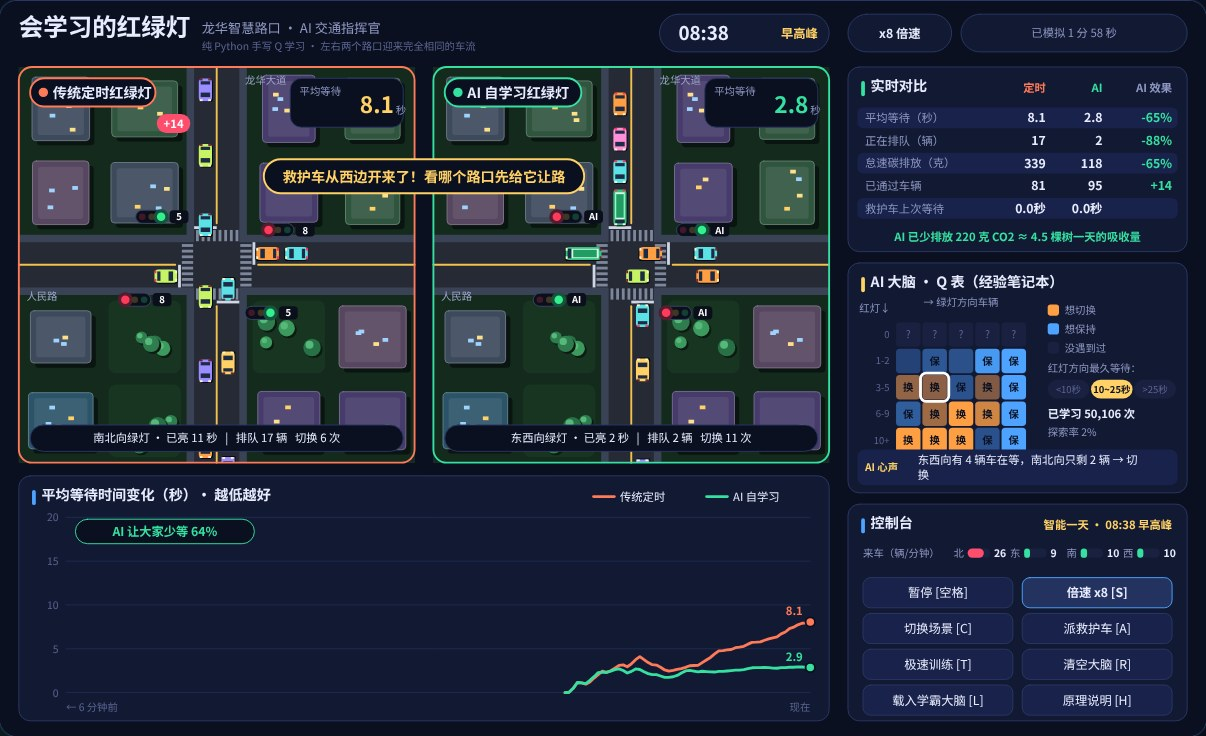
\includegraphics[width=\linewidth]{../docs/images/demo_main.jpg}
  \caption{作品主界面（网页版，早高峰 8 倍速）。左：定时信号灯；右：AI 信号灯；两路口迎来完全相同的车流。
  右侧面板依次为实时对比、AI 的 Q 表热力图与“AI 心声”、控制台；下方曲线为平均等待时间。}
  \label{fig:main}
\end{figure}

% ====================================================================
\section{相关工作}

\textbf{定时与感应控制。}Webster 公式\cite{webster1958}根据流量计算最优周期，是定时控制的经典方法；
SCOOT\cite{hunt1981}、SCATS\cite{sims1980}等系统利用检测器在线调整配时，但依赖人工设计的规则与参数。

\textbf{强化学习信号控制。}Abdulhai 等\cite{abdulhai2003}较早将 Q 学习用于单路口信号控制，证明了其自适应能力。
DeepMind 用深度 Q 网络（DQN）玩 Atari 游戏时提出的\textbf{经验回放}\cite{lin1992,mnih2015}能显著提高样本利用率和训练稳定性。
本作品在表格型 Q 学习中引入经验回放，并通过实验验证了其作用（第~\ref{sec:ablation} 节）。

% ====================================================================
\section{系统设计}

系统按职责分为五层（图~\ref{fig:arch}），上层只依赖下层的接口：
交通仿真不知道谁在指挥它，控制器不知道画面怎么画，绘图代码不知道自己画在哪里。
这样改动任何一层都不会影响其他层，也让同一份代码可以运行在四种环境中。

\begin{figure}[h]
\centering
\begin{tikzpicture}[
  layer/.style={draw=black!40,rounded corners=3pt,fill=softgray,minimum width=4.2cm,minimum height=0.9cm,align=center,font=\small},
  outbox/.style={draw=inkblue,rounded corners=3pt,fill=inkblue!8,minimum width=2.4cm,minimum height=0.8cm,align=center,font=\small},
  arr/.style={-{Stealth[length=2.2mm]},black!55,thick}]
  \node[layer] (sim) {交通仿真\\\footnotesize traffic.py};
  \node[layer,above=0.35cm of sim] (ctl) {控制器 + 安全规则层\\\footnotesize controllers.py};
  \node[layer,right=0.5cm of ctl,fill=aigreen!10,draw=aigreen] (brain) {AI 大脑：Q 学习\\\footnotesize brain.py};
  \node[layer,above=0.35cm of ctl] (world) {对比实验场 / 训练\\\footnotesize world.py, scenario.py};
  \node[layer,above=0.35cm of world] (render) {绘图指令清单\\\footnotesize render.py, ui.py};
  \node[outbox,above left=0.6cm and -1.2cm of render] (tk) {电脑窗口\\\footnotesize tkinter};
  \node[outbox,right=0.25cm of tk] (web) {网页 / 手机\\\footnotesize Pyodide};
  \node[outbox,right=0.25cm of web] (vid) {介绍视频\\\footnotesize Pillow};
  \draw[arr] (ctl) -- (sim);
  \draw[arr] (ctl) -- (brain);
  \draw[arr] (world) -- (ctl);
  \draw[arr] (render) -- (world);
  \draw[arr] (render.north) -- (tk.south);
  \draw[arr] (render.north) -- (web.south);
  \draw[arr] (render.north) -- (vid.south);
\end{tikzpicture}
\caption{系统分层结构。箭头表示“调用 / 依赖”。绘图层只输出与平台无关的指令清单，由三种前端分别绘制。}
\label{fig:arch}
\end{figure}

% ====================================================================
\section{方法}

\subsection{交通仿真}
每条进口车道上的车辆按顺序排列，第 $i$ 辆车只用车头位置 $s_i$ 和速度 $v_i$ 描述。
受 Gipps 安全跟车思想\cite{gipps1981}启发，每一步先求出车辆前方“必须停下的位置” $L_i$
（前车车尾减最小间距 $g_0$，或红灯时的停止线 $s_{\text{stop}}$），再保留与速度成正比的时间车距 $h$：
\begin{equation}
  d_i = L_i - h\,v_i - s_i,\qquad
  v_i^{\text{safe}} = \sqrt{2\,b\,\max(d_i,0)},
\end{equation}
\begin{equation}
  v_i \leftarrow
  \begin{cases}
    \min\!\big(v_i + a\,\Delta t,\; v_i^{\max},\; v_i^{\text{safe}}\big), & v_i^{\text{safe}} > v_i,\\
    \min\!\big(v_i^{\max},\; v_i^{\text{safe}}\big), & \text{否则},
  \end{cases}
  \qquad s_i \leftarrow \min\!\big(s_i + v_i\Delta t,\; \max(s_i, L_i)\big).
\end{equation}
其中 $a$、$b$ 为加速度和最大减速度。第二式中的截断保证车辆\textbf{永不追尾、永不越过红灯停止线}。
黄灯时，若剩余距离满足 $s_{\text{stop}}-s_i \ge v_i^2/(2b_c)$（$b_c$ 为舒适减速度）则停车，否则通过，与真实驾驶相同。
取 $h=0.45$\,s 时，一条车道的饱和流率约为 1 辆/秒，接近真实路口。

信号灯是一个状态机：绿灯 $\to$ 黄灯（2\,s）$\to$ 全红清空（1\,s）$\to$ 另一方向绿灯。
控制器只能“申请切换”，是否允许由信号灯根据最短绿灯（4\,s）判断。

\subsection{马尔可夫决策过程建模}
\textbf{状态。}采用以当前绿灯为参照的\textbf{相对视角}：
\begin{equation}
  s = \big(\,\beta_q(n_g),\; \beta_q(n_r),\; \beta_w(w_r)\,\big),
\end{equation}
$n_g$、$n_r$ 分别为绿灯方向和红灯方向尚未通过停止线的车辆数，$w_r$ 为红灯方向等待最久的车辆的等待时间。
$\beta_q$ 把车数分为 $\{0\},\{1,2\},\{3..5\},\{6..9\},\{10+\}$ 五档，$\beta_w$ 把等待时间分为 $<10$\,s、10～25\,s、$>25$\,s 三档，
共 $5\times5\times3=75$ 个状态。相对视角使南北向学到的经验可直接用于东西向，状态数减半。

\textbf{动作。}$a\in\{\text{保持},\,\text{切换}\}$，AI 在绿灯亮满 4\,s 后每秒决策一次。

\textbf{奖励。}奖励为等待车辆“着急程度”的相反数在动作持续期间的积分：
\begin{equation}
  r = -\frac{1}{10}\int_{t_0}^{t_0+\tau}\;\sum_{j\in\mathcal{W}(t)}\Big(1+\frac{w_j(t)}{30}\Big)\,\mathrm{d}t ,
\end{equation}
$\mathcal{W}(t)$ 为此刻正在等待的车辆集合，$w_j$ 为第 $j$ 辆车已等待的秒数。
每多等 30 秒着急程度加 1，使 AI 不会为了减少排队总数而让少数车辆一直等待（公平性）。

\subsection{半马尔可夫 Q 学习}
“保持”只持续 1\,s，而“切换”要经过黄灯与全红，下一次决策至少在 7\,s 之后，两个动作持续时间不同。
因此采用半马尔可夫决策过程的更新形式\cite{bradtke1995}，用动作实际持续的秒数 $\tau$ 计算折扣：
\begin{equation}
  Q(s,a) \leftarrow Q(s,a) + \alpha_n\Big[\, r + \gamma^{\tau}\max_{a'}Q(s',a') - Q(s,a) \Big],
  \label{eq:q}
\end{equation}
其中 $\gamma=0.95$（每秒）。这样切换带来的约 3 秒“谁都不能走”的损失会真实地进入回报，AI 自己学会“不要乱切换”。

\textbf{自适应学习率。}第 $n$ 次遇到某状态时取 $\alpha_n=\max(0.1,\,1/n)$：
初次遇到的路况完全采信新经验（学得快），见多后稳定在 0.1（不被偶然事件带偏）。

\textbf{探索。}采用 $\varepsilon$-贪心策略，$\varepsilon=\max\!\big(\varepsilon_{\min},\,0.3\,e^{-N/400}\big)$，$N$ 为累计学习次数：
新大脑多探索，经验越多越自信。展示时 $\varepsilon_{\min}=0.02$。

\textbf{经验回放。}每条经验 $(s,a,r,s',\tau)$ 存入容量 5000 的回忆库（满后随机替换），
每学习一条新经验，再随机抽取 $K=20$ 条旧经验按式~\eqref{eq:q} 复习一遍，完整流程见算法~\ref{alg:q}。

\begin{algorithm}[t]
\caption{带经验回放的半马尔可夫 Q 学习控制器（每个仿真步调用）}
\label{alg:q}
\begin{algorithmic}[1]
\Require 路口快照；Q 表；回忆库 $\mathcal{M}$；上一次决策 $(s_{\text{prev}},a_{\text{prev}})$
\State 累积奖励 $R \gets R - \frac{1}{10}\sum_{j\in\mathcal{W}}(1+w_j/30)\,\Delta t$，计时 $\tau\gets\tau+\Delta t$
\If{红灯方向有救护车 \textbf{且} 绿灯方向没有} \Comment{安全规则层}
  \State 立即申请切换；丢弃本次经验；\Return
\EndIf
\If{非绿灯阶段 \textbf{或} 绿灯 $<4$\,s \textbf{或} 距上次决策 $<1$\,s} \Return \EndIf
\State 观察状态 $s$
\If{$s_{\text{prev}}$ 存在}
  \State 按式~\eqref{eq:q} 用 $(s_{\text{prev}},a_{\text{prev}},R,s,\tau)$ 更新，学习率 $\alpha_n$
  \State 把该经验存入 $\mathcal{M}$；从 $\mathcal{M}$ 随机取 $K$ 条按式~\eqref{eq:q} 再学一遍（学习率 $\alpha$）
\EndIf
\If{绿灯已亮 $\ge 40$\,s \textbf{且} 红灯方向有车} $a\gets$ 切换 \Comment{最长绿灯规则}
\Else\ $a\gets\varepsilon$-贪心$(Q(s,\cdot))$
\EndIf
\If{$a=$ 切换} 申请切换 \EndIf
\State $(s_{\text{prev}},a_{\text{prev}})\gets(s,a)$；$R\gets0$；$\tau\gets0$
\end{algorithmic}
\end{algorithm}

\subsection{安全规则层}
安全相关的约束不交给 AI “试错”，而由规则层强制执行：
\begin{itemize}
  \item 最短绿灯 4\,s、黄灯 2\,s、全红 1\,s：写在信号灯状态机中，AI 只能申请，无法违反；
  \item 最长绿灯 40\,s：另一方向有车时必须轮换，保证不会有车辆被无限期“饿死”；
  \item 救护车优先：检测到红灯方向有救护车时立即切换，为生命通道让路。
\end{itemize}
即“AI 负责优化，规则负责兜底”，这也是在现实中使用人工智能应有的方式。

\subsection{可解释性}
为让人看懂 AI 的想法，界面实时显示 Q 表热力图：格子颜色表示 $Q(s,\text{切换})-Q(s,\text{保持})$ 的正负与大小，
白框标出当前路况；“AI 心声”把每一次决定翻译为自然语言，如“东西向有 6 辆车在等，南北向只剩 1 辆 $\to$ 切换”。

% ====================================================================
\section{实现}

\subsection{一套代码，四种运行环境}
绘图代码不直接调用任何图形库，而是输出一份与平台无关的\textbf{绘图指令清单}，例如
\verb|["r", x, y, w, h, fill, ...]| 表示一个矩形。四种前端各自把清单画出来：
电脑版用 tkinter；网页版通过 Pyodide 在浏览器中运行\textbf{同一份} Python 代码，再用 HTML canvas 绘制；
手机版在网页版基础上实现了全屏与竖屏自动旋转；介绍视频则用 Pillow 逐帧绘制。
作品本身只依赖 Python 标准库，可在海龟编辑器中直接运行。

\subsection{核心代码}
Q 学习的更新只需几行（\texttt{smartlight/brain.py}）：
\begin{lstlisting}
def _update(self, state, action, reward, next_state, duration, rate):
    v = self.values(state)
    target = reward + (self.gamma ** duration) * max(self.values(next_state))
    td_error = target - v[action]
    v[action] += rate * td_error
    return td_error
\end{lstlisting}

\subsection{参数}
所有可调参数集中在 \texttt{config.py} 中，主要取值见表~\ref{tab:params}。

\begin{table}[h]
\centering\small
\caption{主要参数}
\label{tab:params}
\begin{tabular}{llll}
\toprule
参数 & 取值 & 参数 & 取值\\
\midrule
仿真步长 $\Delta t$ & 1/30\,s（训练 0.1\,s） & 学习率 $\alpha$ & 0.1 \\
时间车距 $h$ & 0.45\,s & 折扣 $\gamma$（每秒） & 0.95 \\
最短 / 最长绿灯 & 4\,s / 40\,s & 回放容量 / 每次复习 $K$ & 5000 / 20 \\
黄灯 / 全红 & 2\,s / 1\,s & 展示探索率 $\varepsilon_{\min}$ & 0.02 \\
定时灯绿灯 & 15\,s（周期 36\,s） & 预训练 & 24 小时虚拟车流 \\
\bottomrule
\end{tabular}
\end{table}

% ====================================================================
\section{实验}

\subsection{实验设置}
\textbf{公平对照。}两个路口共用同一个随机来车源：每辆车在同一时刻、从同一方向、以同样的最高速度到达两个路口（控制变量法），
差别仅在信号控制器。车辆到达服从泊松过程，各方向强度随时刻变化：早高峰（8:00）北向南最大 0.55 辆/秒，
晚高峰（18:20）南向北最大 0.53 辆/秒，深夜约 0.03 辆/秒，模拟龙华的潮汐车流。

\textbf{评价指标。}平均等待时间定义为
\begin{equation}
  \bar W = \frac{\text{所有车辆停车等待的总秒数（含仍在排队的车）}}{\text{到达车辆数}} .
\end{equation}
制作过程中曾只统计“已驶离路口的车辆”，结果 AI 看上去成绩很好；后来发现一直被堵住、开不走的车根本没被计入，
当时的 AI 实际上会让一个方向长期“饿死”。改用上式后问题才暴露出来。\textbf{选对评价指标与写对算法同样重要。}
此外按怠速 1\,s 排放 0.39\,g CO$_2$ 估算排放。

所有实验可用 \texttt{python tools/experiments.py} 复现。

\subsection{主要结果}
表~\ref{tab:main} 与图~\ref{fig:main-bar} 给出预训练 AI（训练 24 小时虚拟车流，学习 22\,643 次）与定时灯在 5 个场景下各运行 1200\,s 的结果（测试时关闭探索与学习）。
AI 在全部场景中获胜，平均等待时间减少 51.0\%～67.3\%，平均 59.7\%；通过车辆数不减反增，早高峰 20 分钟少排放约 3.2\,kg CO$_2$。

\begin{table}[h]
\centering\small
\caption{定时信号灯与 AI 信号灯对比（1200\,s 仿真，随机种子 11）}
\label{tab:main}
\begin{tabular}{lrrrrr}
\toprule
\multirow{2}{*}{场景} & \multicolumn{2}{c}{平均等待（s/辆）} & \multirow{2}{*}{减少} & \multicolumn{1}{c}{通过车辆} & \multirow{2}{*}{少排放 CO$_2$（g）}\\
\cmidrule(lr){2-3}
 & 定时 & AI & & 定时 / AI & \\
\midrule
早高峰   & 10.49 & \textbf{4.15} & 60.4\% & 1237 / 1257 & 3150 \\
晚高峰   &  9.64 & \textbf{3.58} & 62.9\% & 1195 / 1210 & 2884 \\
深夜     &  6.21 & \textbf{2.03} & 67.3\% &  130 / 131  &  215 \\
智能一天 &  5.56 & \textbf{2.39} & 57.0\% &  582 / 583  &  719 \\
平峰     &  4.65 & \textbf{2.28} & 51.0\% &  516 / 517  &  485 \\
\bottomrule
\end{tabular}
\end{table}

\begin{figure}[h]
\centering
\begin{tikzpicture}
\begin{axis}[
  xbar, width=0.82\linewidth, height=6.2cm, bar width=7pt,
  xmin=0, xmax=12, xlabel={平均等待时间（秒/辆）},
  symbolic y coords={平峰,智能一天,深夜,晚高峰,早高峰}, ytick=data,
  y dir=normal, enlarge y limits=0.15,
  legend style={at={(0.98,0.04)},anchor=south east,font=\small,draw=none,fill=white},
  nodes near coords, nodes near coords style={font=\scriptsize},
  every axis plot/.append style={draw=none},
  axis lines*=left, xmajorgrids, grid style={black!10}]
\addplot[fill=fixedorange!80] coordinates {(10.49,早高峰) (9.64,晚高峰) (6.21,深夜) (5.56,智能一天) (4.65,平峰)};
\addplot[fill=aigreen] coordinates {(4.15,早高峰) (3.58,晚高峰) (2.03,深夜) (2.39,智能一天) (2.28,平峰)};
\legend{定时信号灯, AI 信号灯}
\end{axis}
\end{tikzpicture}
\caption{五个场景下的平均等待时间。差距在早晚高峰最大（定时灯给两个方向相同绿灯，车多的方向越排越长）；
深夜相对减少最多（AI “有车就放行”）。}
\label{fig:main-bar}
\end{figure}

\subsection{消融实验：经验回放}
\label{sec:ablation}
在不使用经验回放（$K=0$）时我们发现，同样的代码换一个随机种子，训练结果差异很大。
为此用 6 个随机种子各训练 2 小时虚拟车流，比较 $K=0$ 与 $K=20$，每个大脑在 4 个时刻各测试 900\,s（表~\ref{tab:ablation}）。

\begin{table}[h]
\centering\small
\caption{经验回放消融（平均等待，s/辆；\red{红色粗体}表示比定时灯更差）}
\label{tab:ablation}
\setlength{\tabcolsep}{5pt}
\begin{tabular}{c rrrr c rrrr}
\toprule
 & \multicolumn{4}{c}{不回放（$K=0$）} & & \multicolumn{4}{c}{经验回放（$K=20$）}\\
\cmidrule(lr){2-5}\cmidrule(lr){7-10}
种子 & 早高峰 & 平峰 & 晚高峰 & 深夜 & & 早高峰 & 平峰 & 晚高峰 & 深夜\\
\midrule
1 & 5.9 & 2.8 & 5.0 & 2.7 & & 4.3 & 2.5 & 3.1 & 2.8\\
2 & \red{26.7} & 2.9 & 14.7 & 1.3 & & 5.2 & 2.3 & 4.7 & 2.4\\
3 & \red{63.1} & \red{7.6} & \red{26.5} & 1.3 & & 5.0 & 2.4 & 3.3 & 2.7\\
4 & 7.6 & 3.0 & 6.9 & \red{8.4} & & 4.9 & 2.4 & 3.7 & 1.3\\
5 & 4.4 & 2.5 & 4.9 & 2.8 & & 4.8 & 2.6 & 4.8 & 1.3\\
6 & 11.0 & 2.5 & 9.5 & 1.3 & & 4.0 & 2.6 & 3.5 & 1.3\\
\midrule
平均 & 19.8 & 3.6 & 11.3 & 3.0 & & \textbf{4.7} & \textbf{2.5} & \textbf{3.9} & \textbf{2.0}\\
\midrule
定时灯 & 21.5 & 4.8 & 18.7 & 4.7 & & 21.5 & 4.8 & 18.7 & 4.7\\
\bottomrule
\end{tabular}
\end{table}

不回放时，6 个种子中有 3 个在至少一个场景比定时灯更差，最差的早高峰平均等待达 63.1\,s；
使用经验回放后，24 个测试结果\textbf{全部}优于定时灯，且不同种子之间非常接近（早高峰 4.0～5.2\,s）。
经验回放让同样多的经历被反复利用，把稀有但关键的路况（如严重拥堵）记得更牢。

\subsection{从零学习的过程}
图~\ref{fig:curve} 记录了清空大脑后在早高峰边用边学的过程。前 3 分钟 AI 还在摸索，表现不如定时灯；
第 4 分钟起反超，第 10 分钟时 AI 平均等待 7.2\,s，而定时灯已升至 39.2\,s。图~\ref{fig:qtable} 对比了学习前后的 Q 表。

\begin{figure}[h]
\centering
\begin{tikzpicture}
\begin{axis}[
  width=0.82\linewidth, height=6cm,
  xlabel={在线学习时间（仿真分钟）}, ylabel={最近 2 分钟平均等待（秒/辆）},
  xmin=1, xmax=12, ymin=0, ymax=45, xtick={1,...,12},
  legend style={at={(0.5,1.03)},anchor=south,legend columns=2,font=\small,draw=none,/tikz/every even column/.append style={column sep=1.2em}},
  axis lines*=left, ymajorgrids, grid style={black!10}]
\addplot[fixedorange,very thick,mark=*,mark size=1.6pt] coordinates {
 (1,8.76) (2,15.48) (3,23.95) (4,24.41) (5,30.26) (6,35.66) (7,37.58) (8,36.48) (9,36.73) (10,39.24) (11,40.55) (12,40.55)};
\addplot[aigreen,very thick,mark=square*,mark size=1.6pt] coordinates {
 (1,10.32) (2,18.10) (3,24.67) (4,20.79) (5,24.43) (6,28.00) (7,24.16) (8,14.05) (9,8.64) (10,7.24) (11,5.29) (12,6.22)};
\legend{定时信号灯, AI（清空大脑后从零学习）}
\end{axis}
\end{tikzpicture}
\caption{早高峰中从零开始的在线学习曲线（\texttt{World} 种子 9，大脑种子 3）。12 分钟内 AI 共学习 305 次。}
\label{fig:curve}
\end{figure}

\begin{figure}[h]
\centering
\begin{subfigure}{0.49\linewidth}
  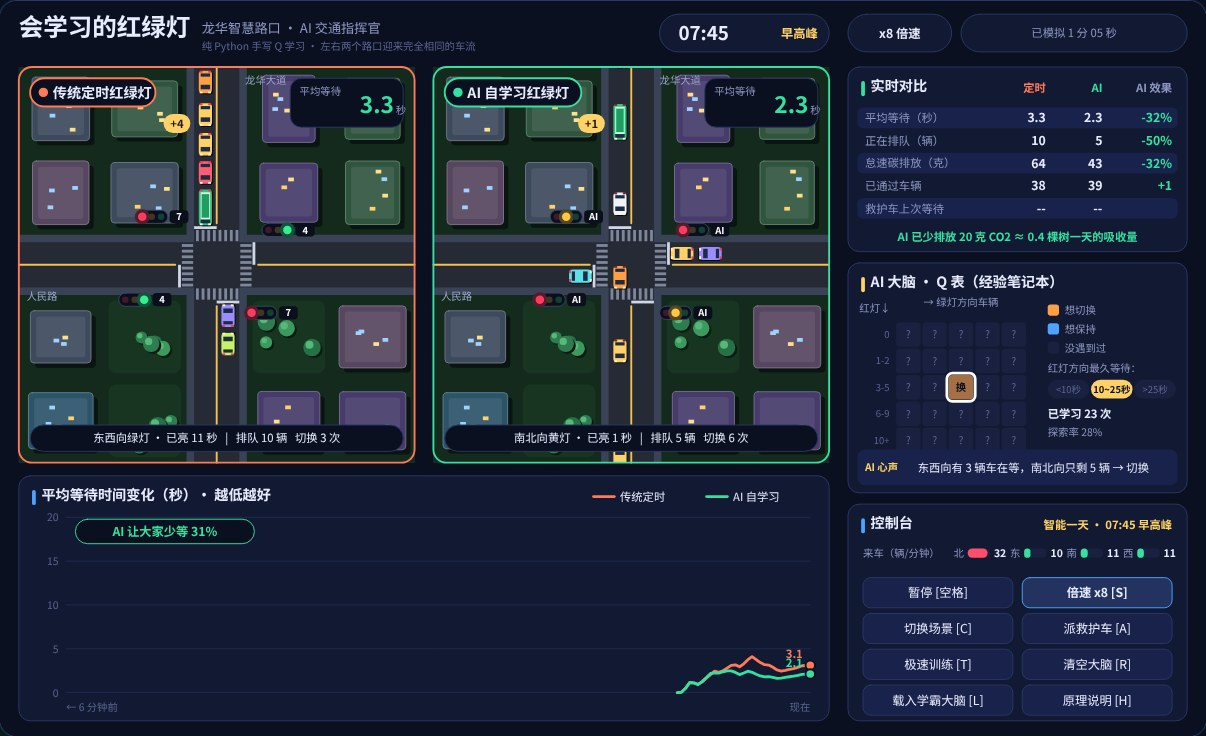
\includegraphics[width=\linewidth]{../docs/images/demo_fresh.jpg}
  \caption{清空大脑后：Q 表全是“？”}
\end{subfigure}\hfill
\begin{subfigure}{0.49\linewidth}
  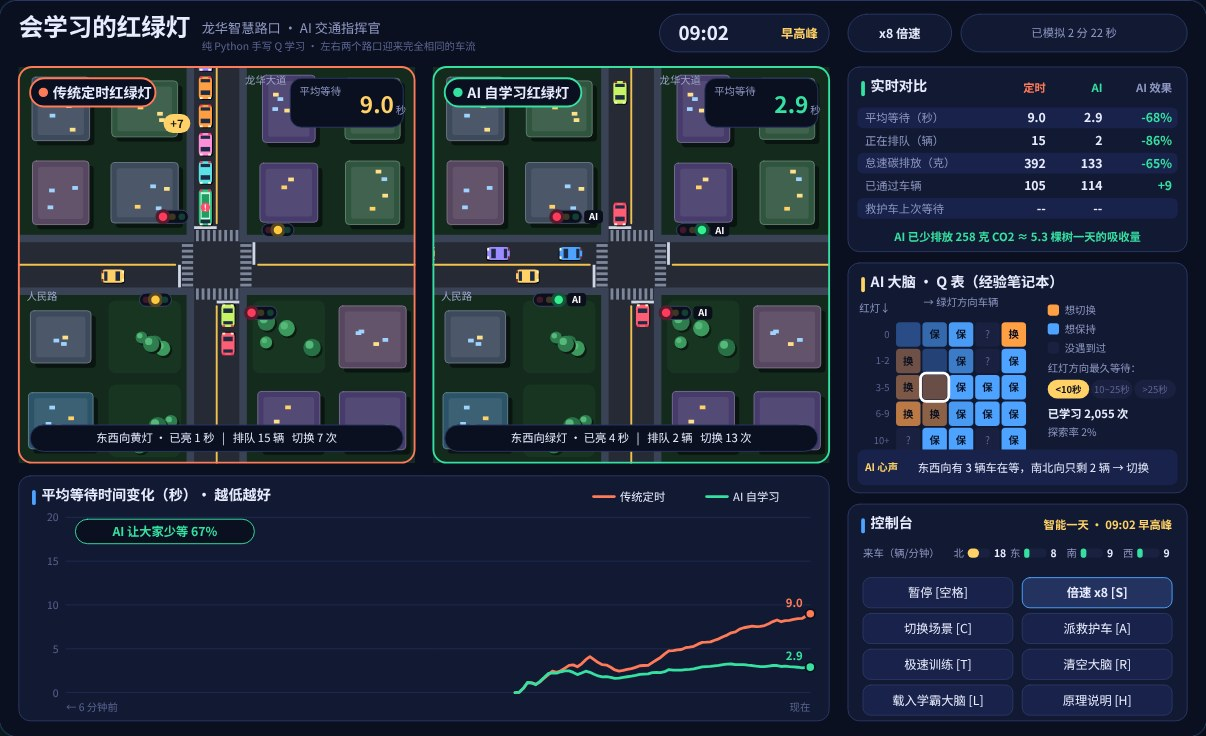
\includegraphics[width=\linewidth]{../docs/images/demo_trained.jpg}
  \caption{“极速训练” 2 小时后：长出规律}
\end{subfigure}
\caption{Q 表的变化（右侧面板中部）。橙色 = 该切换，蓝色 = 该保持：红灯方向车多、绿灯方向车少时切换，反之保持。}
\label{fig:qtable}
\end{figure}

\subsection{测试}
项目包含 9 个自动测试（\texttt{python -m unittest}）：车辆不追尾、不闯红灯；
AI 完全随机决策时安全时间仍被遵守；Q 学习公式数值正确；回忆库容量受限；预训练 AI 在 3 个时刻均比定时灯好 20\% 以上；
救护车优先；界面能正常生成绘图指令。每次推送代码后，GitHub Actions 自动运行测试并发布网页。

% ====================================================================
\section{讨论与反思}

\textbf{收获。}AI 并不神秘，它的“聪明”来自三件事：看什么（状态）、追求什么（奖励）、怎样总结经验（学习算法）。
奖励设计不当时 AI 会“钻空子”，例如只看排队总数时，它会让少数车辆永远等下去。

\textbf{不足与改进方向。}
\begin{enumerate}
  \item 只模拟直行车流，可加入左转、行人过街和更多相位；
  \item 只控制单个路口，可让多个路口的 AI 协同，形成“绿波带”；
  \item 表格型 Q 学习只能处理分档后的路况，可尝试深度强化学习\cite{mnih2015}处理更细致的状态；
  \item 车流为模拟数据，若接入真实交通流量数据，结论将更接近实际应用。
\end{enumerate}

\textbf{AI 伦理。}用 AI 管理公共交通时，效率不是唯一目标，还必须兼顾公平（不让少数人一直等）、
安全（规则兜底）与特殊需要（救护车优先）。

\textbf{作者反思。}（请作者在此用自己的话补充制作过程中的经历与体会。）

% ====================================================================
\section{结论}
本作品用纯 Python 标准库实现了交通仿真与 Q 学习信号控制，并通过公平对照实验证明：
AI 信号灯在五个典型场景中平均减少 59.7\% 的等待时间，经验回放显著提高了学习的稳定性，
安全规则层保证了 AI 的决策始终在安全范围之内。作品支持电脑、网页与手机运行，评委可在线直接体验。

% ====================================================================
\begin{thebibliography}{99}\small
\bibitem{sutton2018} R. S. Sutton, A. G. Barto. \emph{Reinforcement Learning: An Introduction} (2nd ed.). MIT Press, 2018.
\bibitem{watkins1992} C. J. C. H. Watkins, P. Dayan. Q-learning. \emph{Machine Learning}, 8: 279--292, 1992.
\bibitem{lin1992} L.-J. Lin. Self-improving reactive agents based on reinforcement learning, planning and teaching. \emph{Machine Learning}, 8: 293--321, 1992.
\bibitem{mnih2015} V. Mnih, K. Kavukcuoglu, D. Silver, et al. Human-level control through deep reinforcement learning. \emph{Nature}, 518: 529--533, 2015.
\bibitem{bradtke1995} S. J. Bradtke, M. O. Duff. Reinforcement learning methods for continuous-time Markov decision problems. In \emph{Advances in Neural Information Processing Systems 7}, 1995.
\bibitem{abdulhai2003} B. Abdulhai, R. Pringle, G. J. Karakoulas. Reinforcement learning for true adaptive traffic signal control. \emph{Journal of Transportation Engineering}, 129(3): 278--285, 2003.
\bibitem{webster1958} F. V. Webster. \emph{Traffic Signal Settings}. Road Research Technical Paper No. 39, HMSO, London, 1958.
\bibitem{hunt1981} P. B. Hunt, D. I. Robertson, R. D. Bretherton, R. I. Winton. SCOOT---a traffic responsive method of coordinating signals. TRRL Laboratory Report 1014, 1981.
\bibitem{sims1980} A. G. Sims, K. W. Dobinson. The Sydney coordinated adaptive traffic (SCAT) system philosophy and benefits. \emph{IEEE Transactions on Vehicular Technology}, 29(2): 130--137, 1980.
\bibitem{gipps1981} P. G. Gipps. A behavioural car-following model for computer simulation. \emph{Transportation Research Part B}, 15(2): 105--111, 1981.
\end{thebibliography}

% ====================================================================
\appendix
\section{运行方法}
\begin{itemize}
  \item \textbf{电脑：}用海龟编辑器或 IDLE 打开 \texttt{main.py} 直接运行（保持 \texttt{smartlight} 文件夹在同一目录，无需安装任何库）。
  \item \textbf{网页 / 手机：}打开 \url{https://zongruichd-rd.github.io/bisai2/}，手机上点击“全屏演示”。
  \item \textbf{命令行：}\texttt{python train.py}（训练并考试）、\texttt{python -m unittest}（自动测试）、
        \texttt{python tools/experiments.py}（复现本文全部实验）。
\end{itemize}

\section{评分标准对照}
\begin{center}\small
\begin{tabularx}{\linewidth}{>{\bfseries}l X}
\toprule
评分项 & 本作品的对应 \\
\midrule
思想性、规范性 & 用人工智能解决身边的交通拥堵与碳排放问题，关注公平与生命通道；论文、README 齐全，源码均有中文注释 \\
功能与人机交互 & 一键运行；按钮、快捷键、触屏三种操作；开场引导与原理说明；网页与手机在线体验 \\
创新性 & 公平对照实验；Q 表可视化与“AI 心声”；“AI 做梦”极速训练；一套代码四种运行环境 \\
艺术性 & 夜景城市俯视风格；刹车灯、救护车警灯、久等车辆“生气”提示等细节 \\
技术性 & 分层架构；手写半马尔可夫 Q 学习、经验回放、自适应学习率；9 个自动测试；实验可复现 \\
\bottomrule
\end{tabularx}
\end{center}

\end{document}
